\chapter{Dinámica}

\textit{``Si he realizado descubrimientos invaluables ha sido más por tener paciencia que cualquier otro talento.''}\textbf{Sir 
Isaac Newton}
\vspace{1.0cm}

En este apartado se refiere a la Dinámica, la cual es la parte de la Física que estudia o analiza el movimiento desde sus causas 
(fuerzas), es decir, que es lo que genera el movimiento.\\

Las causas que generan el movimiento se denominan fuerzas, entiendiéndose como fuerza a aquella capacidad física que ejerce un 
cuerpo sobre otro y que genera movimiento e incluso deformaciones.\\

La persona que realizó un estudio formidable acerca de Dinámica fue Sir Isaac Newton, y sobre cuyo estudio plasmado en tres leyes 
descansa la base de la Dinámica.
 
\section{Las leyes de Newton:}

Son un total de tres leyes que describen el comportamiento de las fuerzas y como los cuerpos reaccionan ante ellas.

\subsection{Primera Ley de Newton:}

\begin{figure}[ht]
 \centering
 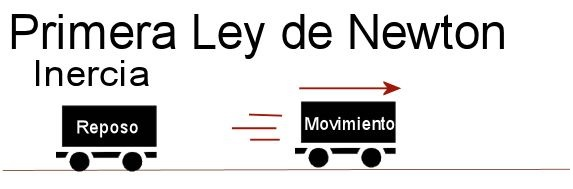
\includegraphics[scale=0.5]{images/primera-ley-de-newton.jpg}
 % cinematica.png: 0x0 px, 300dpi, 0.00x0.00 cm, bb=
 \caption{Ilustración de la primera ley de Newton.}\label{ac}
\end{figure} 

O también conocida como \textbf{Ley de la Inercia\footnote{Oposición o resistencia que presenta un cuerpo para ponerse 
en movimiento.} o de la Masa}, esta ley dice:

\begin{tcolorbox}
"Todo cuerpo que esta en movimiento o en reposo continua en ese estado indefinidamente y solo cambia de estado cuando existe una 
fuerza exterior que modifica la permanencia".
\end{tcolorbox}

Esto implica que si la fuerza resultante aplicado sobre un cuerpo es igual a cero sólo existen dos posibilidades de estado de 
movimiento para ese cuerpo; ya sea el reposo o el MRU. Así, esta ley nos dice que la causa del movimiento es la fuerza, es decir, 
si quiero darle movimiento a un cuerpo debo aplicarle obligatoriamente una fuerza.

\begin{tcolorbox}
Si $\sum \vec{F} = 0$ entonces se tienen reposo ($v = 0$) o MRU ($v =  \text{constante}$)
\end{tcolorbox}

\subsection{Segunda Ley de Newton:}

\begin{figure}[ht]
 \centering
 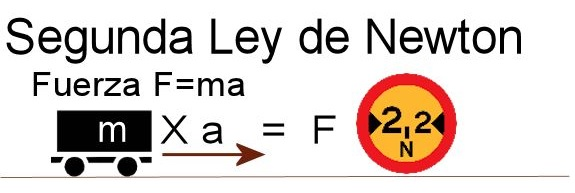
\includegraphics[scale=0.5]{images/segunda-ley-de-newton.jpg}
 % cinematica.png: 0x0 px, 300dpi, 0.00x0.00 cm, bb=
 \caption{Ilustración de la primera ley de Newton.}\label{ac}
\end{figure} 

Tambien conocida como \textbf{Ley de la Fuerza}, y dice:

\begin{tcolorbox}
"Si a un cuerpo de masa $m$ se le aplica una fuerza $\vec{F}$, ésta fuerza le produce una aceleración $a$."
\end{tcolorbox}

Esta aceleración es directamente proporcional a la Fuerza e inversamente proporcional a la masa, y esto se escribe así:

\begin{equation}
\vec{a} \propto \vec{F} \quad y \quad \vec{a} \propto \frac{1}{m}
\end{equation}

Uniendo estas dos proporcionalidades se obtiene que la fuerza es directamente proporcional a la masa y a la aceleración, y así 
queda como ecuación:

\begin{equation}
\vec{F} = m\vec{a} \quad [N]
\end{equation}
donde se ha tomado como constante de proporcionalidad la unidad, y las unidades de la fuerza es el Newton($N$), así mismo para el 
caso de varias fuerzas aplicadas en un cuerpo la ley se generaliza así:

\begin{equation}
\sum \vec{F} = m\vec{a}
\end{equation} 

\subsection{Tercera Ley de Newton}

\begin{figure}[ht]
 \centering
 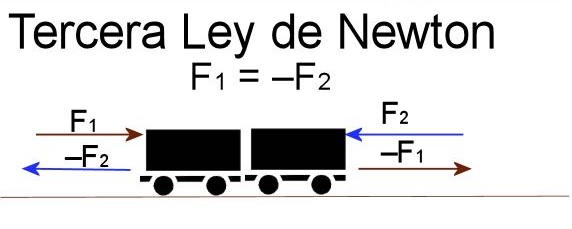
\includegraphics[scale=0.5]{images/tercera-ley-de-newton.jpg}
 % cinematica.png: 0x0 px, 300dpi, 0.00x0.00 cm, bb=
 \caption{Ilustración de la tercera ley de Newton.}\label{ac}
\end{figure}

A esta ley se la conoce como la \textbf{ley de la acción y reacción}, y dice:

\begin{tcolorbox}
''En el Universo las fuerzas nunca aparecen solas, sino en parejas donde una la acción y la otra la reacción, estás fuerzas son 
de igual tamaño pero de sentido contrario".
\end{tcolorbox}

\begin{equation}
\vec{F_{\text{acción}}} = -\vec{F_{\text{reacción}}}
\end{equation}

Es importante descatar que la fuerza de acción y reacción actuan sobre cuerpos diferentes no sobre el mismo.\\

Para abordar problemas de dinámica un poco complejos es importante definir bien algunos tipos de fuerza comunes:

\subsection{El Peso:}

El peso es la fuerza gravitatoria que actúa sobre un objeto que tiene masa ($g$). El peso es causado por la acción del campo 
gravitatorio local sobre la masa del cuerpo. Por ser una fuerza, el peso se representa como un vector, definido por su módulo, 
dirección y sentido, aplicado en el centro de gravedad del cuerpo y dirigido aproximadamente hacia el centro de la Tierra.\\

Clásicamente se calcula así:

\begin{equation}
\vec{P} = m\vec{g}
\end{equation}

\begin{figure}[ht]
 \centering
 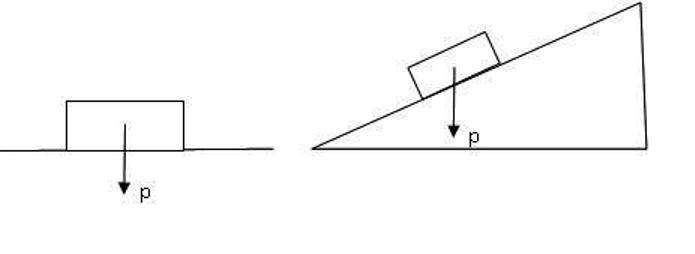
\includegraphics[scale=0.4]{images/peso.jpg}
 % cinematica.png: 0x0 px, 300dpi, 0.00x0.00 cm, bb=
 \caption{Ilustración de la dirección del peso en dos casos diferentes.}\label{ac}
\end{figure}

\subsection{La fuerza normal ($\vec{N}$):}

Es la fuerza que ejerce una superficie sobre un cuerpo apoyado sobre ella. Esta es de igual magnitud y dirección, pero de sentido 
contrario a la fuerza ejercida por el cuerpo sobre la superficie.La fuerza normal es una fuerza de contacto. Si dos superficies 
no están en contacto, no pueden ejercer fuerza normal una sobre la otra.\\

La fuerza normal es la fuerza que las superficies ejercen para prevenir que los objetos sólidos se atraviesen entre sí. Ésta 
fuerza siempre es perpendicular a la superficie de contacto.

\begin{figure}[ht]
 \centering
 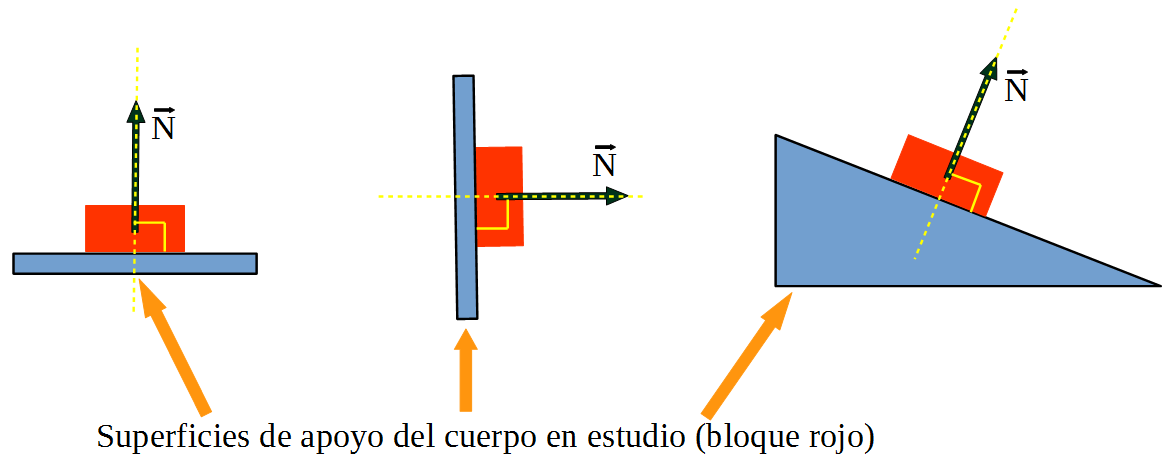
\includegraphics[scale=0.2]{images/fuerzanormal.png}
 % cinematica.png: 0x0 px, 300dpi, 0.00x0.00 cm, bb=
 \caption{Ilustración de la dirección de la fuerza normal en diferentes casos.}\label{ac}
\end{figure}

\subsection{Fuerzas de tensión ($\vec{T}$):}

Son aquellas fuerzas que se transmiten a tráves de cuerdas o hilos cuando se los tensiona.

\begin{figure}[ht]
 \centering
 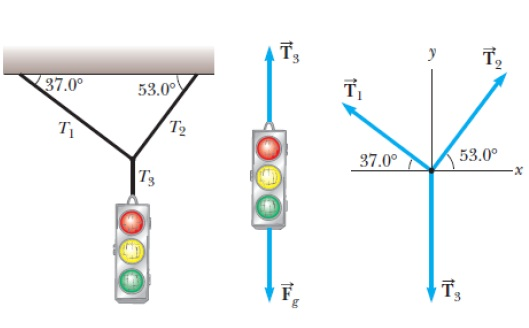
\includegraphics[scale=0.7]{images/tensiones.jpg}
 % cinematica.png: 0x0 px, 300dpi, 0.00x0.00 cm, bb=
 \caption{Ilustración de las tensiones sobre unas cuerdas que sostienen un semáforo.}\label{ac}
\end{figure}

\subsection{Fuerza de rozamiento:}

\begin{figure}[ht]
 \centering
 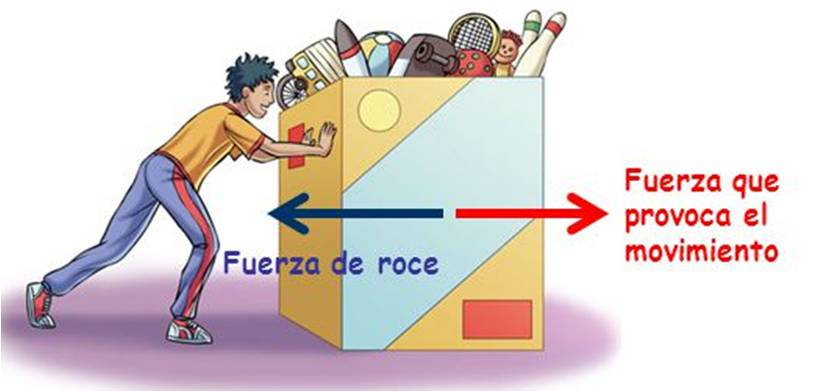
\includegraphics[scale=0.5]{images/fuerza-rozamiento.jpg}
 % cinematica.png: 0x0 px, 300dpi, 0.00x0.00 cm, bb=
 \caption{Ilustración de la fuerza de rozamiento.}\label{fr}
\end{figure}

Se trata de aquella fuerza que se origina cuando dos superficies en contacto se deslizan una sobre otra, debido a que las 
superficies, aún las que se consideran pulidas son extremadamente rugosas a escala microscópica. Es decir, esta fuerza es la que 
se opone al movimiento relativo entre ellas. Esta fuerza es de tipo disipativa, es decir, cuando esta se genera también se genera 
una pérdida de energía que se convierte en calor.\\

Esta fuerza de fricción se comporta de tal manera que cumple con los siguientes postulados básicos:\\

\textbf{a.} La resistencia al deslizamiento tangencial entre dos cuerpos es proporcional a la fuerza normal ejercida entre los 
mismos.
\textbf{b.} La resistencia al deslizamiento tangencial entre dos cuerpos es independiente de las dimensiones de contacto entre 
ambos.\\

La fuerza de fricción ($f_r$) en forma general se calcula de la siguiente manera:

\begin{equation}
f_r = \mu N
\end{equation}
  
donde $\mu$ es una constante adimensional\footnote{Se dice adimensional a aquellas cantidades que no poseen unidades de medida.} 
de llamada coeficiente de rozamiento que depende de la naturaleza de las superficies de rozamiento, que es además un número entre 
0 y 1, además, $N$ es la fuerza normal. Esta fuerza se opone al movimiento relativo al movimiento, por cuanto tendrá una 
dirección opuesta a este movimiento.  
    
\subsubsection{Tipos de Rozamiento:}

Existen dos tipos de rozamiento o fricción, la fricción estática ($f_{rs}$) y la fricción cinética ($f_{rk}$).\\ 
 
\textbf{Fuerza de fricción estática:}\\

Es la resistencia que se debe superar para poner en movimiento un cuerpo con respecto a otro que se encuentra en 
contacto. Se calcula así:

\begin{equation}
f_{rs} = \mu_e N
\end{equation}
donde $\mu_s$ es el coeficiente de rozamiento estatico.\\

\textbf{Fuerza de rozamiento cinética:}\\

Es la resistencia, de magnitud considerada constante, que se opone al movimiento pero una vez que este ya comenzó.

\begin{equation}
f_{rk} = \mu_k N
\end{equation}
donde $\mu_k$ es el coeficiente de rozamiento cinético.

\begin{figure}[ht]
 \centering
 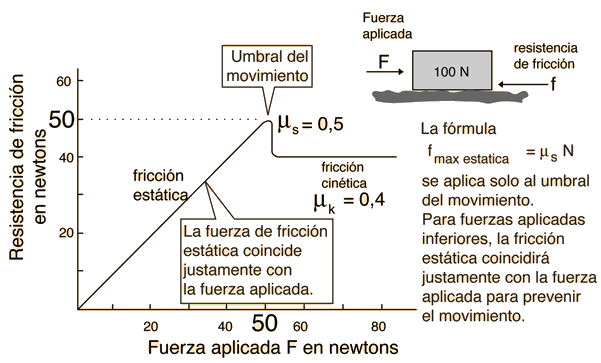
\includegraphics[scale=0.4]{images/fsta.png}
 % cinematica.png: 0x0 px, 300dpi, 0.00x0.00 cm, bb=
 \caption{Ilustración del comportamiento de la fuerza de fricción.}\label{frb}
\end{figure}

En la figura \ref{frb} se puede apreciar como actua el rozamiento cuando se mueve un cuerpo desde el reposo, primero se genera 
fuerza de rozamiento estática ($f_{rs}$) que se va incrementando desde cero hasta un valor máximo donde se supone que el cuerpo 
que se quiere mover comienza a moverse, luego esta fuerza de rozamiento disminuye en valor teniéndose de hecho a lo que se llama 
fuerza de rozamiento cinético ($f_{rk}$).

\section{Diagrama de cuerpo libre:}

Para la resolución de sistemas dinámicas usualmente se usa una técnica llamada el diagrama de cuerpo libre que consiste en un 
boceto de un objeto de interés despojado de todos los objetos que lo rodean y mostrando todas las fuerzas que actúan sobre el 
cuerpo.\\

Consiste en colocar la partícula en el origen de un plano de coordenadas, y representar a las fuerzas que actúan sobre ella por 
medio de los vectores correspondientes, todos concurrentes en el origen. La mayor aplicación de los DCL es visualizar mejor el 
sistema de fuerzas que actúan sobre un cuerpo; además, se identifican mejor las fuerzas pares, como la de acción - reacción y las 
componentes de las fuerzas.\\

Si en un sistema existen dos o más cuerpos de interés, éstos se deben separar y cada uno tiene un DCL propio con sus respectivas 
fuerzas actuando.

\begin{figure}[H]
 \centering
 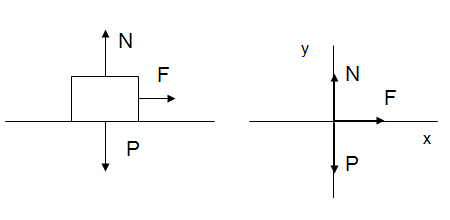
\includegraphics[scale=0.6]{images/cuerpo-libre.png}
 % cinematica.png: 0x0 px, 300dpi, 0.00x0.00 cm, bb=
 \caption{Ilustración de un ejemplo de diagrama de cuerpo libre.}\label{frb}
\end{figure}

\subsection{Problemas de Dinámica}

\begin{enumerate}
 \item Una fuerza neta de 7.5 kN dirigida hacia el oeste actúa sobre un auto de carreras de 1208 kg. ¿A qué velocidad acelerará 
el auto?

\item  ¿Cuál es la masa de un cuerpo, si
 al aplicarle una fuerza de 200 N le produce una aceleración de $40 m/s^2$?

\item  ¿Cuánto tiempo deberá actuar
 una fuerza de 250 N sobre un cuerpo de 12,5 kg para lograr detenerlo si va a una velocidad 
de
 720 km/h?

 \item Un automóvil, con una masa de 1485 kg viaja hacia el sur a 116 km/h, disminuye su velocidad en 10.25 segundos. ¿Cuál es la 
magnitud y la dirección de la fuerza neta que actuó en el camión?

\item Un ascensor pesa 400 Kg. ¿Qué fuerza debe ejercer el cable hacia arriba para que suba con una aceleración de $5 m/s^2$?.

\item Una pelota de fútbol de 550 g de masa adquiere una
 velocidad de 70 m/s mediante un puntapié de 0,2 s de duración, ¿qué 
fuerza recibió la pelota?

\item Una locomotora de 8000 kg de masa tira de un tren de 40000 kg a lo largo de una vía nivelada y lo mueve con una aceleración 
de $1,2 m/s^2$. ¿Con qué aceleración tiraría a un tren de 16000 kg?

\item Resover el problema anterior si la vía descrita tiene un ángulo de $12^\circ$ con respecto a la horizontal.

\item  Una grúa eleva una masa m = 800 kg
 mediante un cable que soporta una tensión de 12000 N. ¿Cuál es la máxima aceleración 
con que
 se puede elevar?

\item Un vehículo de 150 kg de masa se mueve en línea recta a 70 km/h. ¿Qué fuerza debe aplicarse en forma constante para que 
reduzca su velocidad a 20 km/h durante los siguientes 10 segundos de aplicada la fuerza?

\item Calcula la fuerza que habrá que realizar para frenar, hasta detener en 10 segundos un trineo que se mueve a 50 km/h.

\item ¿Cómo cambia la el valor de la aceleración que adquiere un cuerpo si se duplica su masa y se reduce a la mitad el módulo de 
la fuerza aplicada sobre el mismo?.

\item Un vehículo de 800 kg se mueve en un tramo recto y horizontal de autovı́a a 72 km/h. Si por una averı́a deja de funcionar 
el motor y se detiene a los 100 m, calcula la fuerza de rozamiento.

\item ¿Cuál es la masa de un cuerpo, si al aplicarle una fuerza de 420 N de produce una aceleración de $8.4 m/s^2$ ?

\item ¿Cuánto tiempo deberá actuar una fuerza de 80 N sobre un cuerpo de masa de 12.5 kg para lograr detenerlo si va a una 
velocidad de 720 km/h?

\item ¿Cuál es la fuerza necesaria para que un móvil de 1500 kg, partiendo de reposo adquiera una rapidez de $2 m/s^2$ en 12 s?

\item Calcular la masa de un cuerpo, que estando de reposo se le aplica una fuerza de 150 N durante 30 s, permitiéndole recorrer 
10 m. ¿Qué rapidez tendrá al cabo de ese tiempo?

\item  Una auto se mueve a una 
velocidad de 36 km/h, y de pronto debe frenar hasta detenerse antes de cruzar con un semáforo en 
rojo que se ubica a 0,1 km. Determine la fuerza de frenado si el auto tiene una masa de 500 kg.

\item  Si una fuerza se aplica a un 
cuerpo de masa $m$ éste adquiere una aceleración. Si la misma fuerza se aplica a un cuerpo 
de 
masa $2m$, ¿Cuál sería su aceleración?

\item Calcular la magnitud de la aceleración que produce una fuerza cuya magnitud es de 50 N a un cuerpo cuya masa es de 13,000 
gramos.

\item Determinar la magnitud de la fuerza que recibe un cuerpo de 45 kg, la cual le produce una aceleración cuya magnitud es de 
$7 
m/s^2$.

\item Una bala de 0,25 g de masa sale de un cañón de un rifle con una velocidad de 350m/s. ¿Cual es la fuerza promedio que se 
ejerce sobre la bala mientras se desplaza por el cañón de 0.8 m de longitud del rifle?

\item Un carrito de juguete de 3 kg parte del reposo y se mueve una distancia de 4 m en 2 s bajo la acción de una fuerza 
constante 
única.Encuentre la magnitud de la fuerza. 

\item ¿Cuál es la fuerza necesaria para que un móvil de 1700 Kg, partiendo de reposo adquiera una rapidez de $2 m/s^2$ en 12.4 s?

\item Un protón tiene una masa de $1,7 \times 10^{−27} kg$ y se mueve con una velocidad de $2 \times 10^8 m/s$. ¿Qué fuerza será 
necesaria para reducir su velocidad a $10^8 m/s$ en 0.0001 s?

\item Calcular la velocidad final con la que un bloque de masa 10 kg llega a la parte inferior de un plano inclinado de 20 cm 
de largo y 15 cm de alto. Considérese que no hay fuerzas de rozamiento y que la el valor de la aceleración de la gravedad
igual a $10 m/s^2$.

\item Dos bloques de masas $m_1 = 20 kg$ y $m_2 = 8 kg$, están unidos mediante una cuerda homogénea inextensible que pesa 2 kg. Se
aplica al conjunto una fuerza vertical hacia arriba de 560 N. Calcular: a) La aceleración del conjunto; b) Las fuerzas que actúan 
en los extremos de la cuerda.

\item Un astronauta percibe que se aleja lentamente de la estación espacial y la cuerda que lo conecta está rota. En sus manos 
tiene un equipo de 5 kg. ¿Qué podría hacer el astronauta de forma rápida para intentar volver a la estación espacial?     

\end{enumerate}
